
\subsection{Grain Geometry - Thomas Satterly}

A simple study was conducted on the grain geometry by varying the initial inner diameter and length of a cylindrical grain. This case was considered without the AeroValve as to simplify the parameter sweep, but also gain insight on the effects the AeroValve has on feasible grain geometry. The significant results of this study are shown in Figure \ref{fig:grainParamSweep}


\begin{figure}[H]
    \centering
    \begin{subfigure}[b]{0.45\textwidth}
        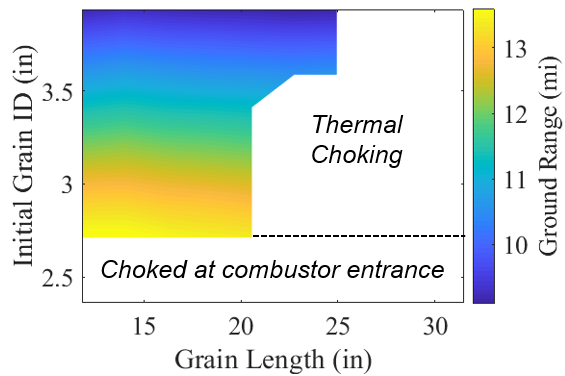
\includegraphics[width=\textwidth]{ParameterSweeps/figures/grainRange.png}
        \caption{Ground Range: Initial Grain ID vs. Length}
        \label{fig:grainParamSubRange}
    \end{subfigure}
    \hfill
    \begin{subfigure}[b]{0.45\textwidth}
        \centering
        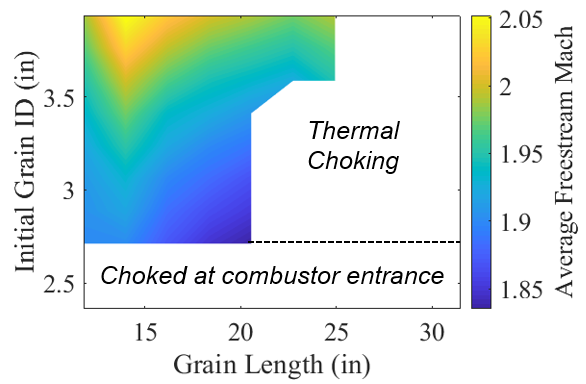
\includegraphics[width=\textwidth]{ParameterSweeps/figures/grainMach.png}
        \caption{Average Freestream Mach: Initial Grain ID vs. Length}
        \label{fig:grainParamSubMach}
    \end{subfigure}
    \caption{Results of grain geometry parameter sweep.}
    \label{fig:grainParamSweep}
\end{figure}

The results shown in Figure \ref{fig:grainParamSweep} are course, but still present meaningful and insightful results. The initial grain inner diameter is limited to approximately 2.75 inches by the flow choking at the combustor entrance, as is represented by the horizontal line in the subfigures \ref{fig:grainParamSubRange} and \ref{fig:grainParamSubMach}. The results also show that the grain length is limited somewhat by thermal choking as the flow increases in temperature down the combustor. While the exact relationship of the feasible grain length for a given initial inner diameter is not made clear due to the coarseness of the parameter sweep, it is reasonable to say that the maximum grain length for a desirable grain lies somewhere near 20 inches. 

The contour plots presented in Figure \ref{fig:grainParamSweep} also show how maximizing ground range pushes the grain geometry to its feasibility limits, specifically the initial inner grain diameter, but at the sacrifice of the average freestream Mach. A smaller initial inner grain diameter translates to more fuel, leading to a greater burn time and ground range, but also a lower average freestream Mach as a result of the extra weight lifted by the booster and lower air mass flow rate at the SFRJ drop condition. Further optimization is clearly needed, as the inlet could be sized more appropriately to these near-optimal conditions, and the addition of an AeroValve could benefit the overall SFRJ performance.